\subsubsubsubsection{ConcreteVehicle}
\begin{figure}[h]
\centering
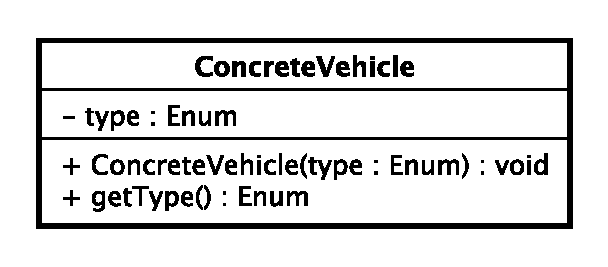
\includegraphics[scale=0.6,keepaspectratio]{images/solution/concrete_vehicle.eps}
\caption{App::Active::ConcreteVehicle}
\label{fig:sd-app-concrete-vehicle}
\end{figure}
\FloatBarrier
\begin{itemize}
  \item \textbf{Description} \\
It represents an entity that only moves on roadways.
  \item \textbf{Attribute}
  \begin{itemize}
    \item \texttt{- type: Enum} \\
Each vehicle has a type \{ car, motorcycle, sidecar \}.
  \end{itemize}
  \item \textbf{Operation}
  \begin{itemize} 
    \item \texttt{+ ConcreteVehicle(type: Enum)} \\
Creates a vehicle specifying its type.
    \item \texttt{+ getType() : Enum} \\
Returns the type of the concrete vehicle.
  \end{itemize}
\end{itemize} 
